The main objective of the technical risk assessment is to determine the reliability compared to the possible (functional or financial) consequences per specific event. To be able to determine any of these reliabilities, a definition of reliability should be stated. In this case, reliability is formulated as:
"The probability that a specific (part of a) subsystem will function without endangering the level zero requirements over the expected lifetime". 

Next to formulating the definition of reliability, it should be noted that the determined reliabilities in this section are relative reliabilities, i.e. the probability that a particular subsystem outperforms another subsystem with the same core function in terms of reliability. Hence, no absolute values of reliability are determined in this section. The relative reliabilities allow for comparison material during the trade-off between multiple design options. 
The risk assessment analysis is divided into four main sections: 
\begin{enumerate}[I]
	\item Ground segment (before vehicle leaves Earth's atmosphere)
	\item During mission
	\item Measurement protocol
	\item Post-mission
\end{enumerate}
The possible events, with their respective reliability, are outlined in these sections and after that the expected consequences are shortly explained. 

\section{Ground segment}
\label{blTRAGs}
\begin{enumerate}[A]
	\item  \textbf{\textit{Financial}} \\\\
\textit{A1. Insufficient funds or low market-demand}\\
The approximate costs are determined in the cost budget. The mission data and the final results can be very interesting for a vast number of commercial companies and research or educational facilities. Every space mission is created for at least one specific (user-demanded) requirement. This third party is responsible for covering the cost. Since the space mission is developed after this request is set, the probability that there will be insufficient funds is low (especially when more than one company can be considered as the user). However, the consequence can be severe if the funds are not enough to start or continue the development. 

	\item  \textbf{\textit{Technological readiness}} \\\\
\textit{B1. Technology for level zero requirements are not available}\\
If the technology for measuring, detecting or processing the level zero requirements is 	not available at present, the requirements can't be met and alternatives should be revised 	(or the mission should be terminated). In our case, the technical readiness level of the 	payload is relatively high and hence has a high reliability. If, however, the specific 	payload would have a low technical readiness level, the mission should be terminated or 	delayed. Therefore, it has important consequences to the mission.

	\item  \textbf{\textit{Launch}} \\\\
\textit{C1. Total launch failure}\\
Total failure indicates complete failure of launch vehicle and all laser swarm 	constellation components. Needless to say, the reliability is relatively low; however, the consequences of this event are catastrophic.

\textit{C2. Partial launch failure}\\
Partial launch failure indicates non-complete failure of laser swarm constellation components, i.e. some of the satellites (emitters or the receiver) can still perform core tasks. Considering historical launch data, the reliability that no partial failure will occur during launch is relatively high. The consequence can be very different, depending on which part (or what fraction) of the constellation can't perform its core task. If one of the receivers will be destroyed, the level zero requirements might still be achievable. However, if the emitter is (partially) destroyed, the mission will surely be endangered. 

\textit{C3. Delayed vehicle launch}\\
Delaying the vehicle launch isn't particularly a problem from the technological side of the mission; however, it will affect the financial situation. Next to the fact that the data and results are delayed, extra costs will be imposed due to an increase in launch vehicle pad costs, extra personnel costs and others. The reliability of this event is actual not that high, since it is dependent on a lot of criteria like third-party companies, the weather, and atmospheric properties. The consequences are mainly financial.

\section{During mission}
\label{blTRADm}
	\item  \textbf{\textit{Orbit accuracy }} \\\\
\textit{D1. One or more satellites are in a wrong orbit.}\\
After launch and orbit initializing, it is possible one or more of the satellites are in a wrong orbit. If this deviation from the desired orbit is relatively small, the ADCS subsystem should be able to cope with this minor error and set the orbit in its right orbit. If the altitude error is large, major altitude changes should be imposed. Assuming a low to moderate error, the consequence is not really severe if the ADCS system is working properly. The chance of actually putting a satellite in the wrong orbit is also pretty small.

In the next section, the reliability of the ADCS subsystems is compared. Assuming a non-hybrid spacecraft, i.e. a spacecraft which uses one of the ADCS subsystems considered in the design option tree, the consequences of failure are equal for all subsystems and thus shall not be inspected individually. The consequences are severe considering not only the loss of pointing accuracy, but also a decrease in vehicle stability and the total failure of controllable altitude control.  	

	\item  \textbf{\textit{Altitude and control determination }} \\\\
\textit{E1.Passive systems}\\

\textit{E1a. Gravity-gradient.}\\
The gravity gradient technique is only dependent on gravity fluctuation in nadir direction, which makes it relatively reliable.

\textit{E1b. Passive magnetic.}\\
The passive magnetic technique is only dependent on magnetic fluctuation near a celestial body. Since this is the only dependency, the technique is really reliable.

\textit{E1c. Zero momentum.}\\
The zero-momentum technique uses a momentum-bias wheel, initially with no angular velocity. Like with all mechanical systems, the presence of (angular) motion will decrease the reliability (due to possible mechanical failure like static failure, fatigue etc.). The reliability however is pretty high, but lower relative to passive magnetic and gravity gradient.

\textit{E1d. Momentum-bias wheel.}\\ 
The momentum-bias wheel technique uses, like the name already predicts, momentum wheels to dump and correct torques. In that sense it has the same reliability as the zero-momentum subsystem. However, since these momentum wheels are constantly spinning, the reliability is slightly lower than the previous mentioned subsystem.

\textit{E1e. Spin stabilization.}\\
Spin stabilization can be achieved using rotation about one principal axis (single-spin) or two principal axes (dual-spin).  Next to the fact that due to external torques (debris collision, aerodynamic drag) the spacecraft can become unstable, i.e. this subsystem has more dependencies, making it relatively unreliable.

\begin{figure} [h]
	\begin{center}
 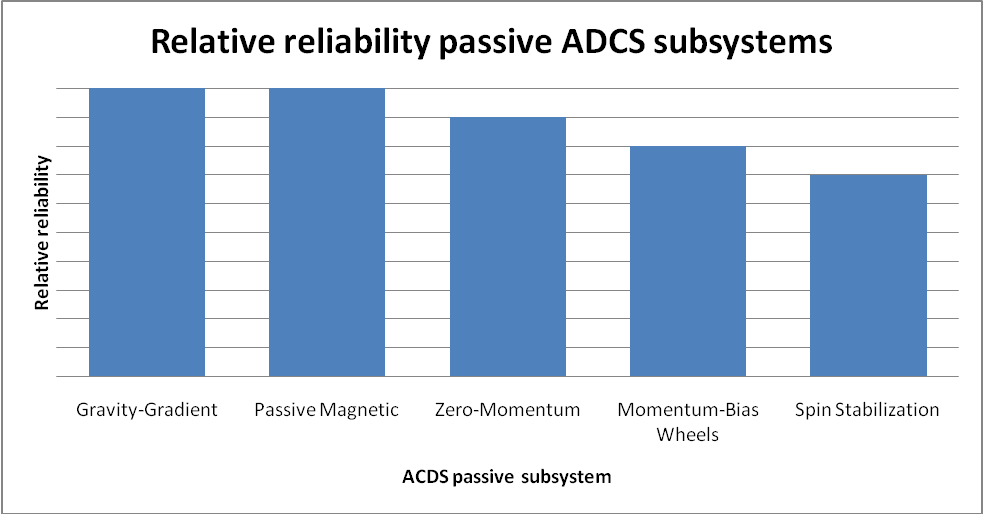
\includegraphics[width=1.0\textwidth,angle=0]{chapters/img/TRA_ADCS_P.png}	
	\caption{Relative reliability passive ADCS subsystems.}
	\label{TRA_ADCS_P}
	\end{center}
\end{figure}

	\item  \textbf{\textit{Active systems}} \\\\
\textit{F1. Actuator}\\

\textit{F1a. Thrusters (hot and cold gas).}\\ 
Multiple-axes thruster systems are very efficient ways for determination and controlling altitude and stability. The system is dependent on fuel consumption, combustion and mechanical properties. Each of these dependencies decreases the reliability. 

\textit{F1b. Reaction and momentum wheels.}\\ 
Mechanical reliability is an import aspect for using active reaction and momentum wheels. 

\textit{F1c. Control Moment gyros.}\\ 
A control-moment-gyro system consists of a spinning rotor and one or more motorized gimbals that tilt the rotor's angular momentum. Mechanical reliability is an import aspect for using this. Since it is also dependent on the motorized gimbals, the reliability is slightly lower than the reaction and momentum wheels.

\textit{F1d. Magnetic torquers}\\ 
The magnetic torquers interact with the Earth's magnetic field, creating compensating torques to induce stability. Reliability is high due to the fact that the magnetic field is known and the system is dependent on a low number of parameters.

\textit{F2. Sensors}\\ 
Assuming a high technical readiness level of the sensors, the reliability is considered high. Also, the consequences of failure are high as the continuation of the mission may be impaired.

\begin{figure} [h]
	\begin{center}
 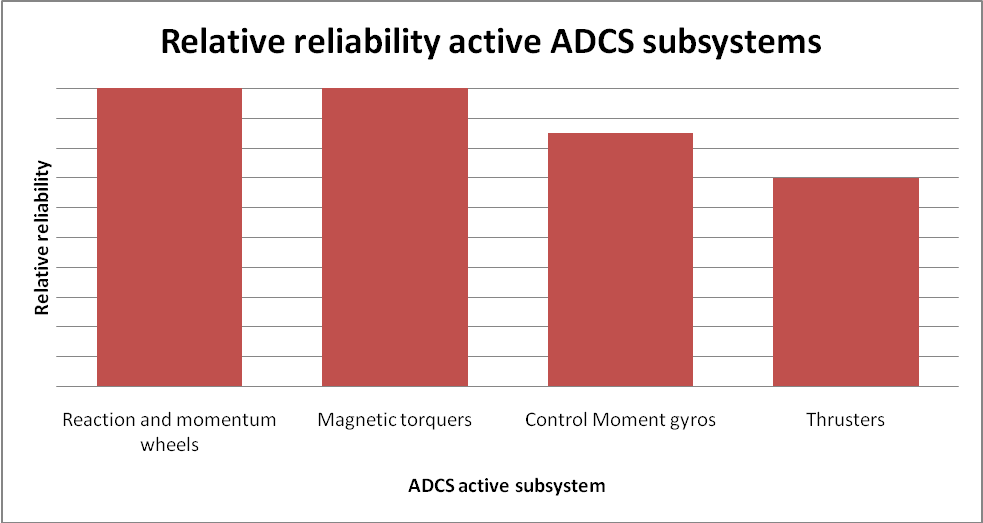
\includegraphics[width=1.0\textwidth,angle=0]{chapters/img/TRA_ADCS_A.png}	
	\caption{Relative reliability Active ADCS subsystems.}
	\label{TRA_ADCS_A}
	\end{center}
\end{figure}

	\item  \textbf{\textit{Electric Power System (EPS)}} \\\\
\textit{G1. Solar Panels}\\

\textit{G1a. Solar panel deflection error or mechanical failure.}\\ 
During launch, the solar panels are retracted to achieve the lowest volume as possible. During the initializing of the mission (assuming the spacecraft is in the right orbit), the solar panels need to be deflected. Errors can occur due to mechanical reasons or external disturbances. The probability of this is pretty low. The consequence can be however that the effective solar panel is decreased and hence a decrease in electrical power will occur. This makes the consequences pretty severe. Any other mechanical failure (broken joints, internal PN-junction failure, maybe even losing an entire solar panel) will have severe consequences as well. 

\textit{G1b. Solar panel characteristics reliability (degradation).}\\ Degradation of solar panels should always be considered during mission development. Since this (should be) known upfront, the consequences are relatively low. The probability of this actually happening is nearly 100 percentage.

\textit{G1c. Severe degradation (due to external phenomenon)}\\ 
Atomic oxygen, hazardous radiation, debris collision and other external factors can influence the performance of the solar panels. Since these are not known from the start, it's difficult to cope with them. The probability of this happening is pretty small, but will have pretty severe consequences.

\textit{G2. Batteries}\\

\textit{G2a. Initial internal failure}\\ 
Considering a high level of technical readiness level, the internal reliability is high. The consequences do alter the functional capacity of the mission, since no energy can be stored if the energy capacity system would completely fail, meaning that during eclipse no energy should be used. 

\textit{G2b. Decrease in capacity}\\ 
Considering a high level of technical readiness level, the reliability is high. Consequences are low, because they are known and should be part of the mission analyses.

\section{Measurement protocol}
\label{blTRAMp}
Since actual measurements are an important level zero requirement, the consequence of the items in the measurement protocol are all really severe. Unless stated otherwise, the consequences in the following section can thus be stated in this way.

\begin{description}
\item[\textit{Measurement}]
\end{description}
	\item\textbf{\textit{Emitter}} \\\\
\textit{H1. Laser pulses can't be sent/ no photon generation}\\ Considering a high level of technical readiness level, the reliability is high.

\textit{H2. Pointing towards nadir}\\
This is dependent on ADCS risks.

\textit{H3. Laser notifies receiver (time adjustment)}\\ 
Considering a high level of technical readiness level, the reliability is high.

\textit{H4. Laser degradation}\\
Laser degradation is dependent on multiple parameters: thermal properties, input power interval, external factors and internal mechanical errors (manufacturing or design errors). However, due to extensive research and development concerning laser technology, the probability of severe laser degradation within the lifetime is relatively low. 

	\item\textbf{\textit{Receiver}} \\\\
\textit{I1. Point towards target} 
This is dependent on ADCS risks.
\textit{I2. Receive and detect photons}\\ 
Considering multiple satellite receivers, the probability of total failure to receive and detect photons using advanced single photon receiving devices (like SILAT, Glass or photon-receiving modules) is negligible. 
\textit{I3. Turn photon into electrical signal}\\ 
Considering a high level of technical readiness level, the reliability is high.

\begin{description}
\item[\textit{Communication}]
\end{description}
	\item\textbf{\textit{Inter satellite communication}} \\\\
\textit{J1. Determine relative position receiver and emitter}\\ 
Considering a high level of technical readiness level, the reliability is high.

\textit{J2. Time differences}\\ 
Considering a high level of technical readiness level, the reliability is high.

	\item\textbf{\textit{Data handling}} \\\\
\textit{K1. Store data/ make data package}\\ 
Considering a high level of technical readiness level, the reliability is high.

\textit{K2. Transmit package}\\ 
Considering a high level of technical readiness level and relative low-tech technology, the reliability is high.

\textit{K3. Interpreted results}\\ 
Historical data comparisons for the interpretation of altimetry missions are sufficient, but not elaborate. However, the reliability is still pretty high.

\textit{K4. Reproduce terrain model}\\
Historical data comparisons for the interpretation of altimetry missions are sufficient, but not elaborate. However, the reliability is still pretty high.
 
	\item\textbf{\textit{Housekeeping/ Ground communication}} \\
\textit{L1. Housekeeping data from ground station to satellite}\\ 
Considering a high level of technical readiness level, the reliability is high.

\textit{L2. Adjusting space segment characteristics}\\ 
Considering a high level of technical readiness level, the reliability is high.

	\item\textbf{\textit{Structural}} \\\\
\textit{M1. Joints}\\ 
Considering a high level of technical readiness level, the reliability is high.

\textit{M2. Connection points}\\ 
Considering a high level of technical readiness level, the reliability is high.

\textit{M3. Thermal limits}\\ 
Thermal limits will alter the characteristics of pretty much all subsystems. However, thermal will be excluded in this analysis.

\textit{M4. Fatigue}\\ 
High-cycle loading is usually not present (except for momentum wheels) and should therefore only play a minor role. The probability is low. The consequences are medium to high if high-cycle loading will lead to fatigue and hence partial failure.

\textit{M5. Electrical overlay failure}\\ 
See EPS

	\item\textbf{\textit{External}} \\\\
\textit{N1. Debris collision}\\ 
Unknown external phenomenon. The probability of this event causing total failure, which is a function of multiple parameters like orbit and celestial position, is low to medium. 

\textit{N2. Dangerous radiation}\\ 
Unknown external phenomenon. The probability of this event causing total failure, which is a function of multiple parameters like orbit and celestial position, is low to medium. 

\textit{N3. Charged particles collision}\\ 
Unknown external phenomenon. The probability of this event causing total failure, which is a function of multiple parameters like orbit and celestial position, is low to medium. 

\textit{N5. Politics or international influence}\\ 
Political decisions or international influences can alter the space mission considerably.  With altimetry missions, the probability of these external influences causing a delayed or complete stop of the mission is negligible. The consequences could be very severe though. 

\textit{N6. Classified information (army)}\\ 
Some parts of the measurement are classified information, for example military ground stations or governmental classified areas. The government and/ or military can pressure the vehicle engineers to keep certain information classified. However, if this is the case, most of the measurements still can be taken and analyzed. So where the probability is medium, the consequences are very low.

\section{Post-mission}
\label{blTRAPm}
	\item\textbf{\textit{Satellite decommission}} \\\\
\textit{O1. Decommission LEO}\\ 
At the end of life the satellites have to be decommissioned to allow new mission to take their place. To decommission satellites in low Earth orbit one could just wait a couple of years and air drag will cause de satellites orbit to degrade to the point they burn up in the atmosphere, so the consequences are low. However, it is desirable to have the satellites burn up faster, so as to remove the risks like satellite collision. The probability to no longer be able to eject the satellite from orbit depends on whether or not its propulsion is still working; as such this probability is low.

\textit{O2. Decommission GEO}\\ 
Satellites in GEO can not be placed in an orbit that will cause them to burn up in the atmosphere because they will cross paths with too many other satellites. Because risk is so high these satellites are instead decommissioned by ejected them from orbit further into space. This way, new GEO satellites can take the place of the swarm. If this in the dead satellites will continue orbiting the Earth, wasting space that can be used by other satellites, as a result the consequence of failure is high. Being able to reposition a satellite depends on the ADCS systems, as such the probability of this event is low.

\begin{figure} [h]
	\begin{center}
 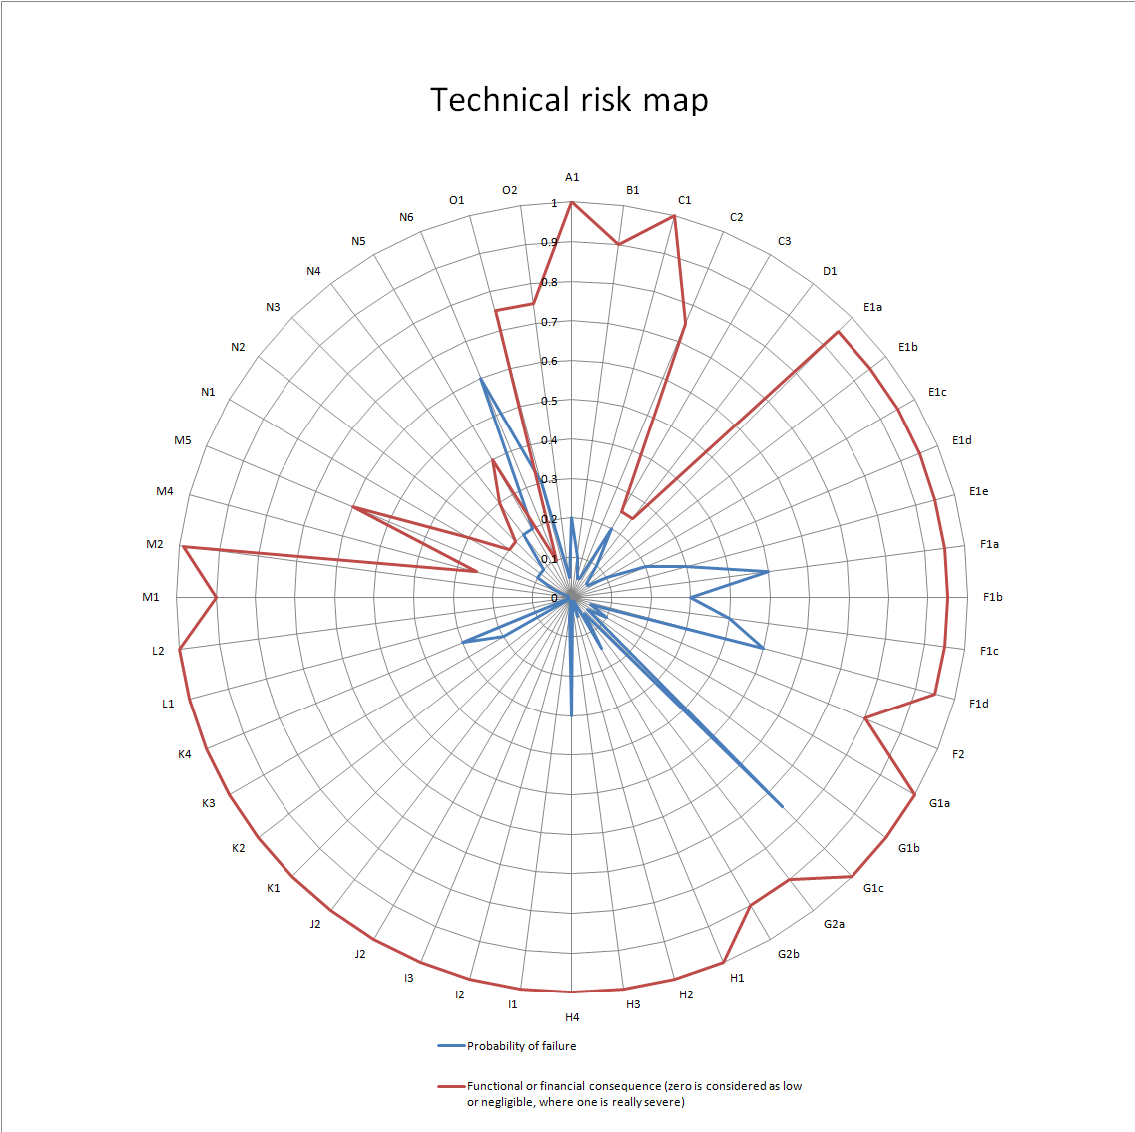
\includegraphics[width=1.0\textwidth,angle=0]{chapters/img/TRA_RM.png}	
	\caption{Technical Risk Assessment}
	\label{TRA_RM}
	\end{center}
\end{figure}

\end{enumerate}